\documentclass[10pt]{exam}
\usepackage[icp]{template-for-exam}
\usepackage{pgfplots}

\title{Introduction to ICP Stations}
\author{Rohrbach}
\date{\today}




\begin{document}
\maketitle
\vspace{1em}

\hrule

\section{Physics}

\vs[2]

\hrule

\vspace{1em}

\section{Classroom Expectations}

\begin{quote}
Important things to remember:


\begin{enumerate}
\item 
\item \vs
\end{enumerate}
\vs

\noindent One question you have:
\vs

\end{quote}

\hrule

\section{Evaluating Expressions}


\begin{center}
	\begin{tikzpicture}
		\draw (0,0) rectangle ++ (7,3);
		\draw (8,0) rectangle ++ (7,3);
		\draw (4,-4) rectangle ++ (7,3);
	\end{tikzpicture}
\end{center}

\vspace{1em}

\pagebreak

\section{Algebra}

\begin{center}
	\begin{tabular}
		{ m{.25\textwidth} | m{.3\textwidth}| m{.25\textwidth} } 
		first equation: & second equation: & third equation:  \\[20em]
	\end{tabular}
\end{center}

\vspace{1em}

\hrule

\section{Graphing}

\begin{center}
	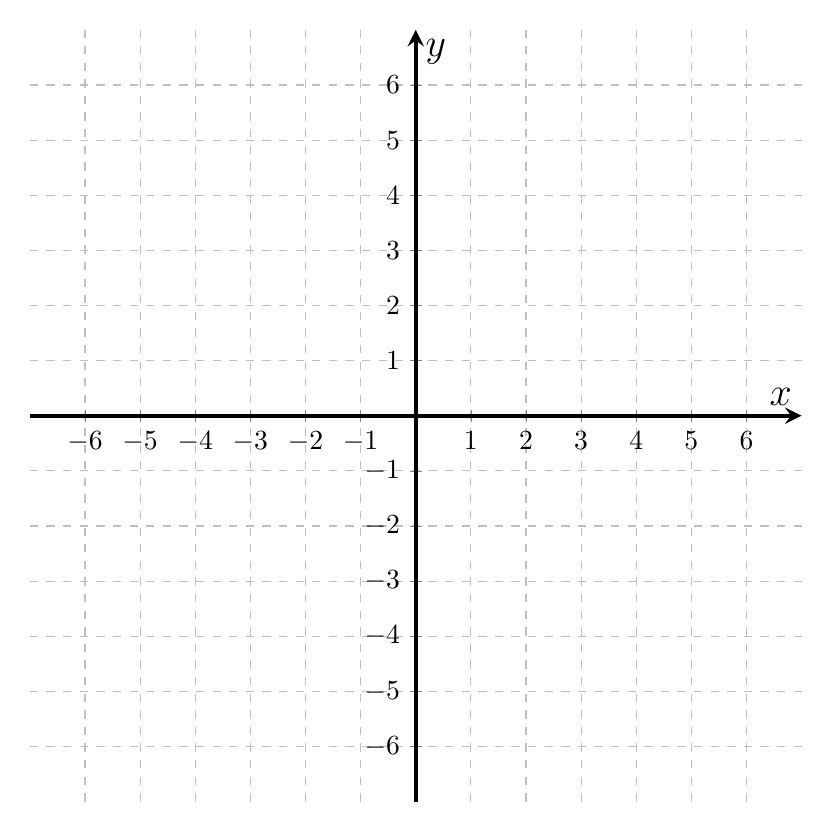
\begin{tikzpicture}
		\begin{axis}[
		    axis lines = center,
	             axis line style = ultra thick,
	             grid style = thin,
		    xlabel={\Large $x$},
		    ylabel={\Large $y$},
		    ymin=-7,
		    ymax=7,
		    xmin=-7,
		    xmax=7,
		    xtick={-6,...,6},
		    ytick={-6,...,6},
	      grid=major,
				grid style = dashed,
				x=.7cm,
				y=.7cm,
		]
		\end{axis}
	\end{tikzpicture}
\end{center}



\end{document}
